\section{First observing run results}

Advanced LIGO's first observing run (O1) lasted from September 12, 2015 - 
January 19, 2016. In this observing run, the first direct detection of 
gravitational waves was achieved with the discovery of two binary black 
hole mergers, GW150914 and GW151226. 

Figure \ref{fig:GW150914} shows a 
filtered time domain representation of the first detection, GW150914, 
with the best estimated 
waveform overlaid on top. Both the signal and the waveform have been 
bandpass filtered to isolate the frequency range where the signal has 
power. Static lines, such as the 60 Hz power line frequency and 
interferometer calibration lines, have been notched out of the data. 
The signal demonstrates the characteristic ``chirp", 
increasing in frequency and amplitude as a function of time as  
expected from a compact binary coalescence. 

\begin{figure}[ht!]
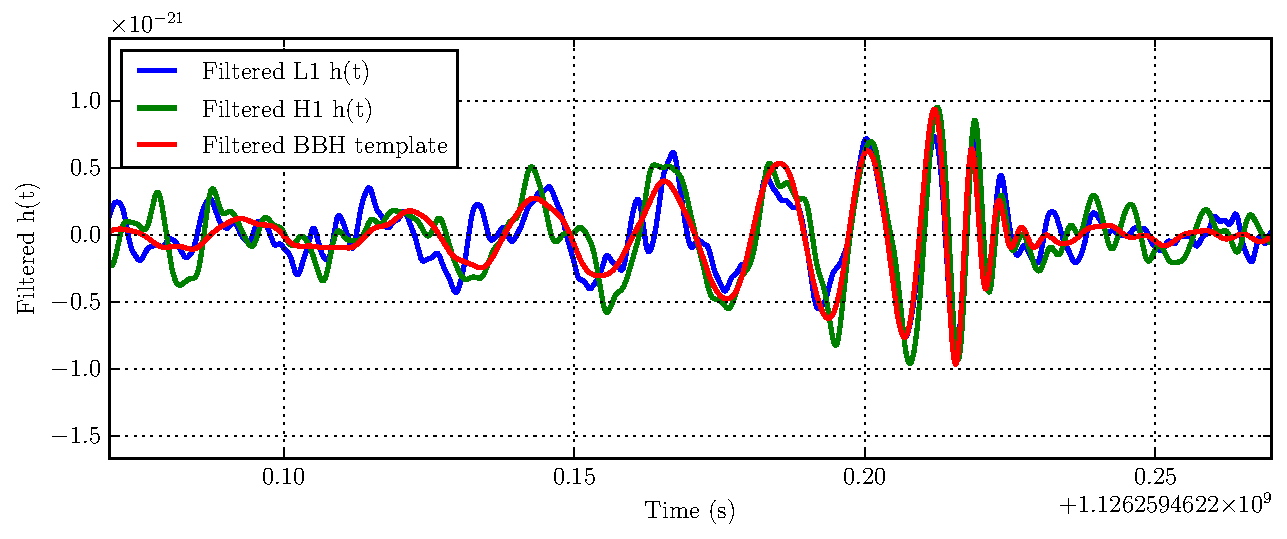
\includegraphics[width=\textwidth]{figures/O1/GW150914-timeseries}
\caption[GW150914 timeseries]{Time domain representation of L1 %
        gravitational wave strain at the time of GW150914. The blue %
        curve is strain, zero-phase bandpass filtered to isolate the %
        frequencies that contain signal. The red curve is a CBC waveform %
        generated using the best estimated parameters. The CBC waveform %
        has been filtered in the same way as the strain curve. The overlap %
        between the two curves is significant, demonstrating many cycles %
        of clear coherence.}
\label{fig:GW150914}
\end{figure}

It is exceptional that GW150914 is visible in the detector data with 
very conservative filtering. Due to the high total mass of the system, 
which is detailed in Table \ref{table:foreground}, the black holes 
of GW150914 coalesced quickly and at a low frequency, spending about 
0.2 seconds in the frequency range that aLIGO is sensitive to. The 
signal was also tremendously loud due to its total mass and relatively 
close distance. 
As a result, the power in the signal is highly localized in time, 
producing a short, loud waveform that is readily visualized.

The other binary black hole signal, GW151226, has a rather different 
morphology. The system that produced GW151226 was roughly three times 
less massive than that of GW150914 and was estimated to have merged 
at a similar distance (see Table \ref{table:foreground}). Due to the 
lower total mass, GW151226 has an overall lower amplitude than GW150914 
and has its power distributed more broadly in time. GW151226 spent about 
2 seconds in the frequency band that aLIGO is sensitive to, which is a 
factor of 10 longer than the duration of GW150914. For these reasons, 
it is not feasible to generate a time domain visualization of the signal. 
However, this is a fantastic demonstration of the value of a 
matched-filter search for CBC signals. The signal-to-noise ratio 
reported by a matched-filter search is an 
integral in the frequency domain that is designed to identify modeled 
signals regardless of their duration.

\section{PyCBC results}

The search for compact binary
coalescences was performed by two parallel search pipelines: PyCBC and 
GstLAL. In addition to these searches for modeled sources, an unmodeled 
burst search, Coherent Wave Burst (CWB), was run to search for coherent 
transient signals in the two Advanced LIGO interferometers. 
All three of these analyses produced consistent results. 
For brevity, we will focus on the results of the PyCBC search pipeline.


\begin{figure}[ht!]%
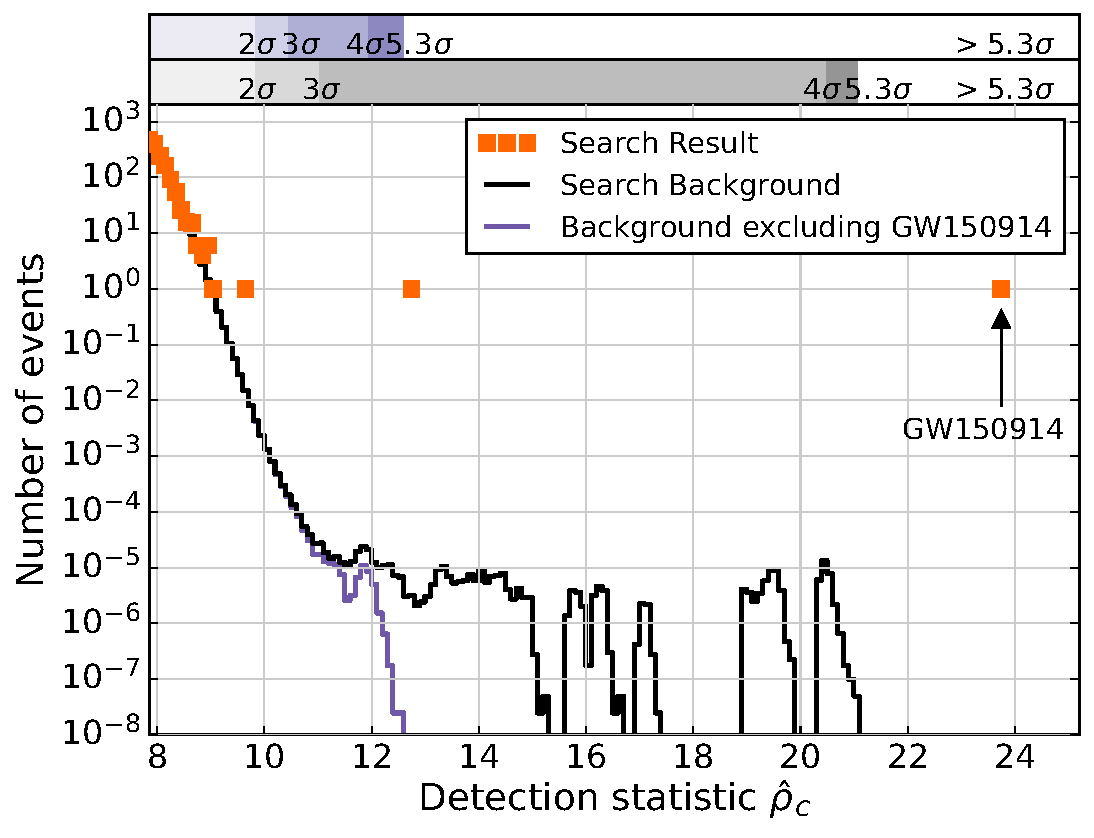
\includegraphics[width=0.8\textwidth]{figures/O1/pycbc_hist_GW150914}
\caption[PyCBC result histograms for GW150914]{Histograms of PyCBC results for GW150914}
\label{fig:pycbc-hist-gw150914}
\end{figure}

How significant was GW151226? We have to remove GW150914 to find out. 
Then Figure \ref{fig:pycbc-hist-gw151226} can tell us!

\begin{figure}[ht!]%
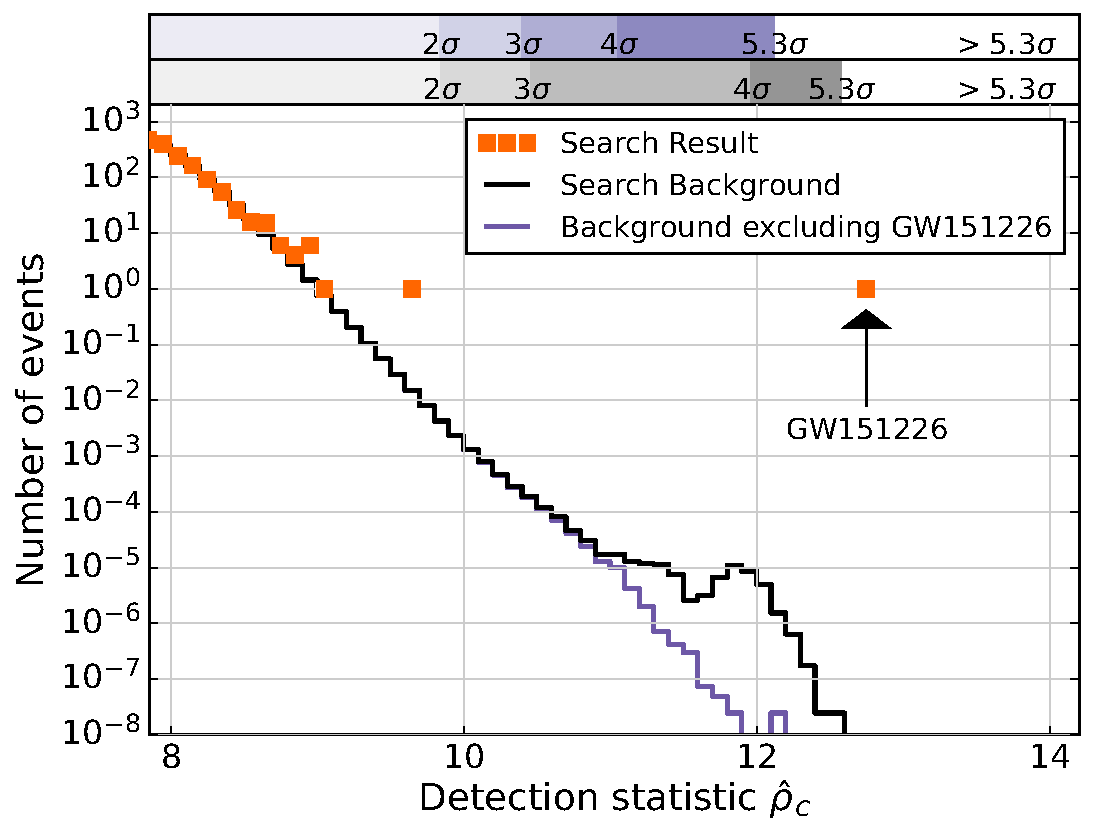
\includegraphics[width=0.8\textwidth]{figures/O1/pycbc_hist_GW151226}
\caption[PyCBC result histograms for GW151226]{Histograms of PyCBC results for GW151226}
\label{fig:pycbc-hist-gw151226}
\end{figure}

\begin{table}[ht!]%
  \begin{center}
    \footnotesize
    \begin{tabular}{ccccccc}
    \hline
    Event & Time(UTC) & FAR ($yr^{-1}$) & $m_1$ ($M_{\odot}$) & $m_2$ ($M_{\odot}$) & $S_{eff}$ & $D_L$ (Mpc) \\
    \hline
    GW150914 & \begin{tabular}{@{}c@{}}14 September \\ 2015 \\ 09:50:45 \end{tabular} & 
    $< 5.8\times10^{-7}$ & $36_{-4}^{+5}$ & $29_{-4}^{+4}$ & $-0.06_{-0.18}^{+0.17}$ & 
    $410_{-180}^{+160}$ \\
    GW151226 & \begin{tabular}{@{}c@{}}26 December \\  2015 \\ 03:38:53 \end{tabular} & 
    $< 5.8\times10^{-7}$ & $14_{-3}^{+9}$ & $8_{-3}^{+2}$ & $0.20_{-0.10}^{+0.21}$ & 
    $490_{-210}^{+180}$ \\
    LVT151012 & \begin{tabular}{@{}c@{}}12 October \\ 2015 \\ 09:54:43 \end{tabular} & 
    0.44 & $23_{-5}^{+18}$ & $13_{-5}^{+4}$ & $0.0_{-0.2}^{+0.3}$ & 
    $1100_{-500}^{+500}$ \\
    \hline
    \end{tabular}
  \end{center}
  \caption[Table of foreground events]{Table of foreground events found in the first %
           observing run. %
           The quoted false alarm rates are calculated by the PyCBC search pipeline. %
           The GstLAL search pipeline reported similar results. % 
           Two binary black hole systems, GW150914 and GW151226, were %
           discovered with a false alarm rate $< 5.8\times10^{-7}$, which is the upper %
           limit on false alarm rate set by the amount of time used in the analysis. %
           A third event, LVT151012, was an interesting foreground event that was not %
           statistically significant to be claimed as a detection, but could be part %
           of a larger gravitational wave population that includes weaker signals.
           } 
  \label{table:foreground}
\end{table}

